\documentclass[12pt,a4paper]{article}
\usepackage[utf8]{inputenc}
\usepackage[russian]{babel}
\usepackage[OT1]{fontenc}
\usepackage{amsmath}
\usepackage{amsfonts}
\usepackage{amssymb}
\usepackage{graphicx}
\graphicspath{{Images/}}
\usepackage[left=2cm,right=2cm,top=2cm,bottom=2cm]{geometry}
\usepackage{calc}
\usepackage{wrapfig}
\usepackage{tikz}
\usepackage{pgfplots}
\usepackage[export]{adjustbox}
\usepackage{setspace}
\usepackage{indentfirst}
\usepackage{subfigure}
\usepackage{multirow}


\title{
1.3.3.

Измерение вязкости воздуха по течению
в тонких трубках
}

\author{Семёнов Андрей Б02-016}

\begin{document}

\date{25 марта 2021г.}
\maketitle
\newpage

\textbf{Цель работы:} экспериментально исследовать свойства течения газов по тонким трубкам при различных числах Рейнольдса; выявить область применимости закона Пуазейля и с его помощью определить коэффициент вязкости воздуха.

\textbf{В работе используются:} система подачи воздуха (компрессор, поводящие трубки); газовый счетчик барабанного типа; спиртовой микроманометр с регулируемым наклоном; набор трубок различного диаметра с выходами для подсоединения микроманометра; секундомер

\section{Теоретический материал}

Работа посвящена изучению течения воздуха по прямой трубе круглого сечения. Движение жидкости или газа вызывается перепадом внешнего давления на концах $\Delta P$ трубы, чему в свою очередь препятствуют силы вязкого (внутреннего) трения, действующие между соседними слоями жидкости, а также со стороны стенок трубы.

Сила вязкого трения как в жидкостях, так и в газах описывается законом
Ньютона: касательное напряжение между слоями пропорционально перепаду
скорости течения в направлении, поперечном к потоку. В частности, если жидкость течёт вдоль оси x,  а скорость течения $v_{x}(y)$ зависит от координаты $y$  в каждом слое возникает направленное по $x$ касательное напряжение.

Величину $\eta$ называют коэффициентом динамической вязкости (или просто вязкостью) среды.

Объёмным расходом (или просто расходом) $Q$ называют объём жидкости,
протекающий через сечение трубы в единицу времени. Величина $Q$ зависит от
перепада давления $\Delta P$, а также от свойств газа (плотности $\rho$ и вязкости $\eta$) и от
геометрических размеров (радиуса трубы $R$ и её длины $L$). Основная задача
данной работы — исследовать эту зависимость экспериментально.

Характер течения в трубе может быть ламинарным либо турбулентным. 

Характер течения определяется безразмерным параметром задачи — числом Рейнольдса

$$ Re = \frac{\rho u a}{\eta}$$, где

$\rho$ - плотность жидкости, $u$ - скорость движения потока, $a$ - характерный размер потока.

Выпишем некоторые теоретические зависимости:

$$P(x) = P_{0} - \frac{\Delta P}{l}x$$

$$u = \frac{Q}{\pi R^{2}} = \frac{U_{max}}{2}$$

$$Q = \frac{\pi R^{4} \Delta P}{8\eta l}$$

$$a_{\text{уст}} \approx 0,2R\cdot Re$$
\newpage

\section{Экспериментальная установка}

\begin{figure}[h!]
	\begin{center}
		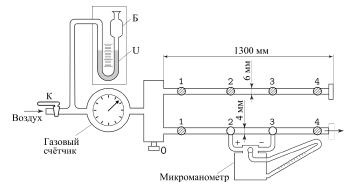
\includegraphics[width = 0.85\textwidth]{Scem_of_facility}
		\caption{Схема экспериментальной установки}
		\label{fig:facility}
	\end{center}
\end{figure}

\section{Выполнение работы}
\indent Оценим расстояние, на котором происходит формирование потока при ламинарном течении.
$a\approx0,2r*Re=0,2*1,95*10^{-2}*1000\approx 40$ (см)

Давление, измеряемое микроманометром, определяется по формуле:
$$P=K*h*9,80665$$
где \\
P $-$ давление в Паскалях \\
$h$ $-$ число делений \\
$K=0,2$ $-$ постоянная угла наклона \\

\begin{table}[h!]
\centering
\begin{tabular}{|c|c|c|}
\hline
              & $d$, мм & $\sigma$, мм \\ \hline
Первая трубка & 5,25    & 0,05         \\ \hline
Вторая трубка & 3,00    & 0,05         \\ \hline
Третья трубка & 3,95    & 0,05         \\ \hline
\end{tabular}
\caption{Внутренние диаметры трубок установки}
\label{tab:facilitys_tube_diam}
\end{table}

\begin{table}[h!]
\centering
\begin{tabular}{|c|c|c|c|c|}
\hline
№ измерения & $\Delta V$, л & $t$, с & $\Delta P$, дел  \\ \hline
1                         &  2                  & 80      &  20    \\ \hline
2                         &  3                  & 78      &  30     \\ \hline
3                         &  5                  & 99      &  40    \\ \hline
4                         &  6                  & 94      &  50     \\ \hline
5                         &  7                  & 99      &  55    \\ \hline
6                         &  8                  & 104    &  60      \\ \hline
7                         &  9                  & 108    &  65       \\ \hline
8                         &  10                & 112    &  70       \\ \hline
\end{tabular}
\caption{Результаты измерения зависимости перепада давления от расхода воздуха, ламинарный режим}
\label{tab:flow_measuring_laminar}
\end{table}


\begin{table}[h!]
\centering
\begin{tabular}{|c|c|c|c|}
\hline
№ измерения & $\Delta V$, л &  $t$, с & $\Delta P$, дел  \\ \hline
1                         & 7                   & 67      & 95    \\ \hline
2                         & 10                 & 88      & 127    \\ \hline
3                         & 11                 & 92      & 151    \\ \hline
4                         & 12                 & 92      & 182     \\ \hline
5                         & 12                 & 83      & 214    \\ \hline
6                         & 15                 & 99      & 243      \\ \hline
7                         & 20                 & 122    & 277       \\ \hline
\end{tabular}
\caption{Результаты измерения зависимости перепада давления от расхода воздуха, турбулентный режим}
\label{tab:flow_measuring_turbulent}
\end{table}


Построим график зависимости давления от расхода:\\
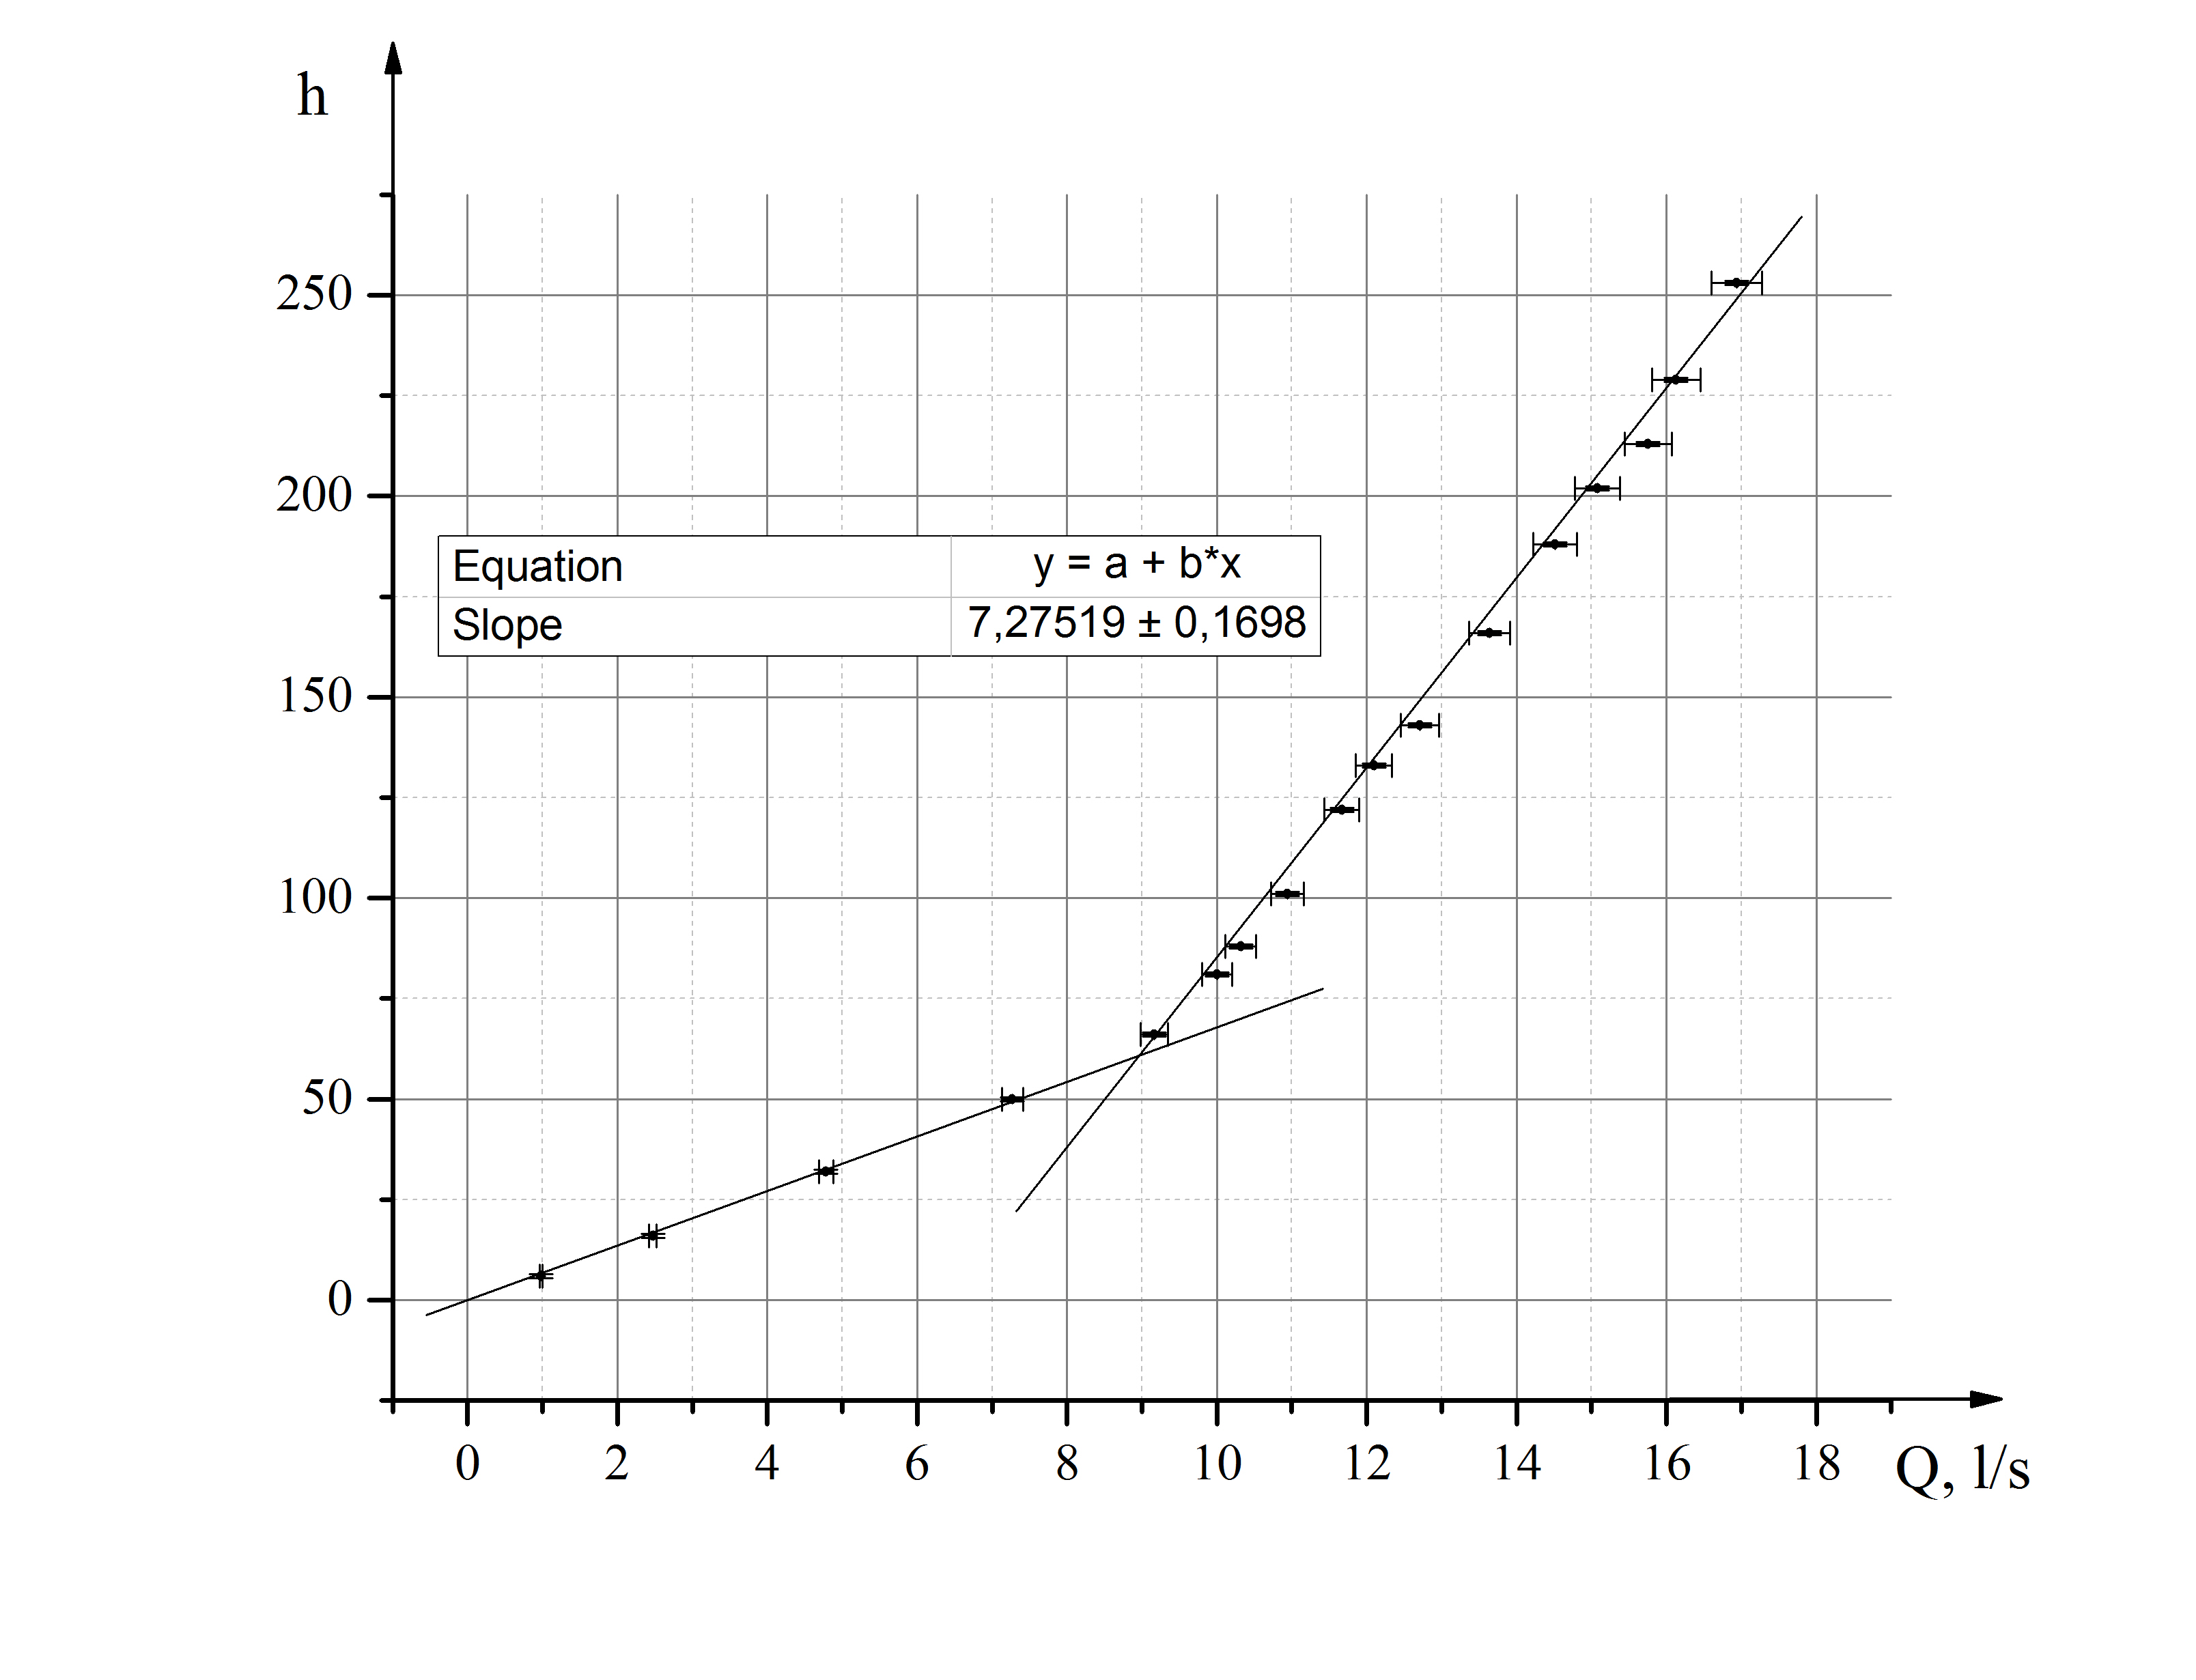
\includegraphics[scale=0.7]{Graph1.jpg}
Выразим искомую вязкость через коэффициент наклона прямой $\alpha$
$$h=\eta*\frac{8l}{\pi r^4K*8,80665}Q=\alpha Q$$
$$\eta = \frac{\pi r^4 K*9,80665 \alpha}{8l}$$
$l=(50,0\pm0,1$) cм \\

$\epsilon_\eta = \sqrt{4\epsilon_R^2+\epsilon_\alpha^2+\epsilon_l^2}=0,03$\\


$\eta =(1,61\pm0,05)*10^{-5}$ кг*м/с \\ 

\ \\


Из графика видно, что ламинарный режим переходит в турбулентный на значениях $(8-9)*10^2 \ $м$^3$/с
$$Re=\frac{Qr\rho}{S\eta}$$
$Re=(980-1100)$


При расходе, заведомо обеспечивающем ламинарность потока измерим распределение давления вдоль трубки:\\
\\
\begin{tabular}{|c|c|c|c|c|c|}
\hline 
l, см & 11,2 & 30 & 40 & 50  \\ 
\hline 
$\Delta P$, дел & 54 & 62 & 73 & 75  \\ 
\hline 
\end{tabular}
\\
\\
\\
Построим график зависимости давления от расстояния: \\
\\
\begin{minipage}[h]{0.69\textwidth}
\begin{tikzpicture}[scale = 1]
\begin{axis}[
    axis lines = left,
    legend style={at={(0.9, 0.3)}},
    xlabel = {$x$, $\text{см}$},
    ylabel = {$\Delta P$, $\text{дел}$},
    xmin=0, xmax=80,
    ymin=30, ymax=80,
	ymajorgrids = true,
	xmajorgrids = true
]
\addplot[
	mark = square, 
	mark options = {
	scale = 1.5, 
	fill = red, 
	},
	ymajorgrids = true,
	xmajorgrids = true,
	color = orange 
]  coordinates {
	(11.2, 54) (30, 62) (40, 73) (50, 75)};
\end{axis}
\end{tikzpicture}
\end{minipage}


\section{Выводы}

\begin{enumerate}
	\item При выполнении данной работы были исследованы различные режимы течения газа по трубкам. На практике получена экспериментальная зависимость разницы давления в различных точках трубки в зависимости от расхода воздуха, идущего через трубку.
	\item Исследовались условия перехода течения из одного режима (ламинарного) в другой (турбулентный).
	\item Полученные зависимости разницы давлений от расхода воздуха согласуются с существующей теорией, описывающей движение газов и жидкостей в различных режимах.
	\item Определено значение вязкости воздуха : $\eta_{\text{эксп}} = \left(1,6 \pm 0,6\right) \cdot 10^{-6}$ Па$\cdot$с, при табличном значении $\eta_{\text{табл}} = \left(1,3 \pm 0,2\right) \cdot 10^{-6}$ Па$\cdot$с. Полученные значения равны в пределах погрешности.
	\item Основной вклад в погрешность итогового значения вязкости внесла погрешность измерения времени, а так же погрешности измерения давлений. Погрешности, связанные с установкой (погрешность линейных размеров установки, диаметра трубок) внесли меньший вклад в итоговое значение погрешности.
	\item Частично подтверждена теоретическая линейная зависимость падания давления с изменением расстояния от края трубки. Также необходимо уточнить, что за время выполнения лабораторной работы температура в комнате понизилась на несколько градусов. 
	\item Подтверждена формула Пуазейля для расхода газа при прохождении через трубку.
\end{enumerate}
\end{document}